\chapter{Java Application}
\label{cha:789}

%generic to go in depth

BPMNPA is a Java Application developed to add new BPMN elements in a Business Process Diagram generated through a PDDL plan. In order to accomplish such objective a few tools has been used, which will be listed below.

\begin{itemize}  
\item Eclipse BPMN2 Modeler: in order to visit the Business Process Diagram and gather valuable information about his structure, the BPMN2 file it is treated as a collection of graphs in which from a starting point, specified from the user, a visit will be executed to map the structure in Java Objects. Eclipse BPMN2 Modeler provides us the Java Classes relative to the BPMN2 elements and allows us to operate on them using the provided methods.

\item LPG-td: a PDDL planner capable of supporting all PDDL1.2 and PDDL2.1 specifications. Its purpose is to generate a plan through the information contained in two PDDL text file, a domain and a problem. The plan generated consists of a list of PDDL actions, time slots and execution times. 

\item Eclipse Modeling Framework: a modeling framework and code generation facility for building tools. The EMF project, in BPMNPA, is being used as support to Eclipse BPMN2 Modeler to load the resource of a BPMN2 file.
\end{itemize}


% specific 

With the support of the tools and plug-ins previously described, the Java application will complete a set of procedures in order to update the BPMN2 file with the new plan.

Firstly, the input parameters will be handled and checked, more on this topic in the next section since BPMNPA requires an extensive number of arguments in input.
Secondly, through EMF and Eclipse BPMN2 Modeler, the resources of the BPMN2 file, provided by the user, will be loaded in the Java application. Such action permits the prototype to analyze the Business Process Diagram with the methods supplied  by the tools.
Thirdly, a graph traversal is executed on the BPD, such visit will return the list of reachable Flow Object. Such list will contain the Flow Objects eligible to set the goal for the PDDL problem. Such list is ordered in base of the priority in which every Flow Object should be considered as goal.

% questa e' complicata
At this point, we have an ordered list of eligible BPMN2 Flow Objects in Java. 
Starting from the elements with higher priority (which are the first elements encountered iterating the ordered-list), for all the elements in the list a plan will be generated until a suitable one is found. 
This is achieved by generating a PDDL problem file, in compliance with the relative BPMN elements, and executing the planner using such file and the proper domain. 
The output produced by LPG-td is evaluated and, if the output contains a suitable plan compliance with the given constraints, then the iteration will stop and the next step is executed, else the iteration continue in search of a valid plan.

After a fitting plan has been found, the planner output will be parsed in order to produce the BPMN2 elements to represent the plan at its best. A list of BPMN2 elements will be created on the base of specific parameters that will be disclosed in section 2.2 and, after creating a backup for the BPMN2 file, the original diagram will be updated with the plan produced.

\begin{center}
\begin{figure}[h!]
		\centerline{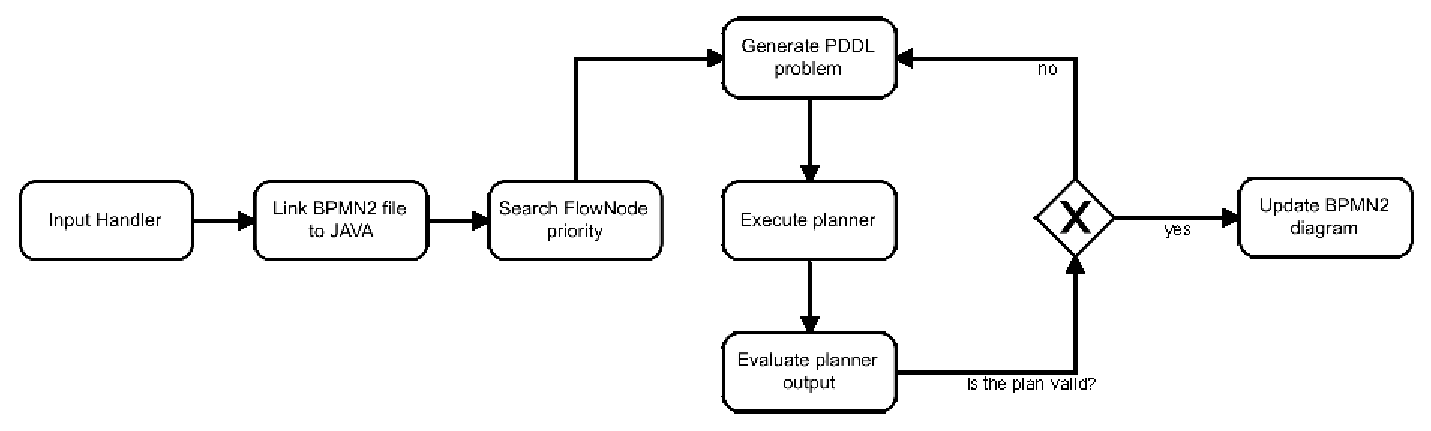
\includegraphics[width=1\textwidth]{diagram.eps}}
		\caption{The execution of BPMNPA}
\end{figure}
\end{center}

\newpage

\section{Input Parameters}
\label{sec:456}

Up to six different input arguments may be required for a correct execution of BPMNPA.
Some of them are mandatory to generate a positive outcome, while the others will allow the user to create more specific plans. The additional arguments allow the user to specify certain parameters, these can be used to modify the plan metrics. 

\paragraph{Mandatory input parameters}
\begin{itemize}

   \item[String] that we will call "planner", which has the aim of specifying the usage of the planner and the address of the executable in the file-system. The string needs to contain the keywords: \texttt{domain}, \texttt{prob} and \texttt{output}. Such keywords will be substituted with the proper sub-strings at run-time. 
   Such solution has been outlined in order to facilitate a future  improvement with the aim to establish a compatibility of BPMNPA with other planners than LPG-td. 
   It is not an easily understandable way to specify the parameter, but it has plenty of versatility and allows the user to specify optional setting for the planner execution. 
   
 	\item[String] that we will call "domain", which has the aim of specifying the path in the file-system of the PDDL domain file. This file needs to contain all the necessary elements to grant the correct execution of LPG-td such as: the name of the domain, the requirements, predicates and actions. If the user intend to use the other available parameters to specify some PDDL metrics, then it is mandatory for the domain file to contain the Functions PDDL Object.
	
	\item[String] that we will call "bpmn", which has the aim of specifying the path in the file-system of the BPMN2 compliance file. 


	\item[String] that we will call "from", which has the aim of specifying the ID of the BPMN Flow Object that will be used to set the initial states and objects in the PDDL problem. This parameter has been designed to allow the user to specify the element where the BPMN simulation (or execution) stops due to an error and cannot restore itself to reach a satisfying state or, more easily, the element from which the user decide to create a new plan. 


	\item[String] that we will call "pddl", which represents the path in the file-system of a directory containing the PDDL representations of the Flow Objects of the Business Process Diagram. 
	Every Flow Object of the BPD should have a PDDL file associated, such file must have as name the ID of the element and no file extension. 
	Furthermore, it is required that the file referring to the BPMN element used in the parameter "from" contains at least the "objects" and the "init" PDDL Objects while the files that represents the other elements must contain at least the "goal" PDDL Object.
	
\end{itemize}

\newpage
\paragraph{Optional input parameters}
\begin{itemize}
	\item[Integer] that we will call "distance", which has the aim of specifying the max number of actions that a plan can contain to be valid. It has been designed to permit the user to specify which aspect has to be prioritize, less actions added to the BPD or a BPD with lesser deviation from the original appearance.
	 
	\item[String] that we will call "max", which has the aim of specifying which metric should be maximized while searching a new plan, to use this argument it is necessary a compliance with the PDDL domain file about metrics and functions.
	
	\item[String] that we will call "min", which has the aim of specifying which metric should be minimized while searching a new plan, to use this argument it is necessary a compliance with the PDDL domain file about metrics and functions.\footnote{Only one between "max" and "min" parameters can be specified at the time.}

\end{itemize}

\begin{lstlisting}[caption=Input example with only mandatory parameters using bash.]
./BPMNPA --planner "./lpg-td -o domain -f prob -out output -n 1" --domain "domain.pddl" --bpmn "file.bpmn2" --from "Task_1" --pddl "./bpmnelements/"
\end{lstlisting}

\begin{lstlisting}[caption=Input example with optional parameters using bash.]
./BPMNPA --planner "./planner/lpg-td -o domain -f prob -out output -n 1" --domain "pddl/domain0.pddl" --bpmn "bpmn/file.bpmn2" --from "StartEvent_1" --pddl "bpmnelements/" --deviation "6" --min "(+ (price) (fuel-usage))"
\end{lstlisting}
	


\section{Transforming Plans into Business Processes}
\label{sec:456}
BPMNPA will return to the user a modified Business Process Diagram, with a new plan drawn in it. 
The new plan is generated by the planner and needs to be parsed and transformed from text to BPMN elements. 
To accomplish this, it is necessary to analyze firstly the structure of the Business Process Diagram and secondly the structure of the PDDL plan. In total, we have identified three principles that we will follow in the transposition from PDDL to BPMN.

\begin{itemize}  
\item The plan generated goes from a Flow Object to another Flow Object and in the initial path between those elements a diverging Exclusive Gateway was present without the relative converging Exclusive Gateway. In this case other plans must be generated setting as goal an element for every other branch of the outgoings Sequence Flow of the diverging Exclusive Gateway.

\item The plan generated contains actions with the same temporal slot, then the representation of those actions will be confined between a diverging Parallel Gateway and a converging Parallel Gateway.

\item Any single action will be represented as a Task element, with a random alphanumeric string as ID and with the action name as Task name.
\end{itemize}


With respect to the three previous guidelines, BPMNPA will create Task element, Parallel Gateway element and Sequence Flow element. Each Flow Object (Task and Gateway) will be linked through a Sequence Flow with another BPMN2 element, no isolated object will be created.

\newpage

\begin{lstlisting}[caption=Planner output example. In this case the first and the second actions can be executed in any order.]
0:   (ACTION0 A) [1]
0:   (ACTION0 B) [1]
1:   (ACTION1 C) [1]
2:   (ACTION2 A B) [1]
2:   (ACTION2 B C) [1]
2:   (ACTION2 C A) [1]
3:   (ACTION3 A B C) [1]
\end{lstlisting}


\begin{figure}[h!]
	\centering
	\begin{subfigure}[b]{0.7\linewidth}
    	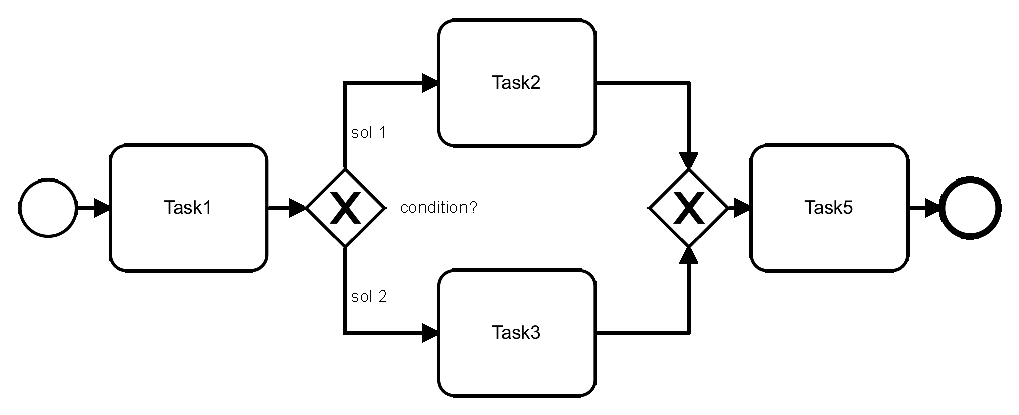
\includegraphics[width=\linewidth]{examplepre.eps}
    	\caption{The initial Business Process Diagram.}
  	\end{subfigure}
	\begin{subfigure}[b]{1\linewidth}
    	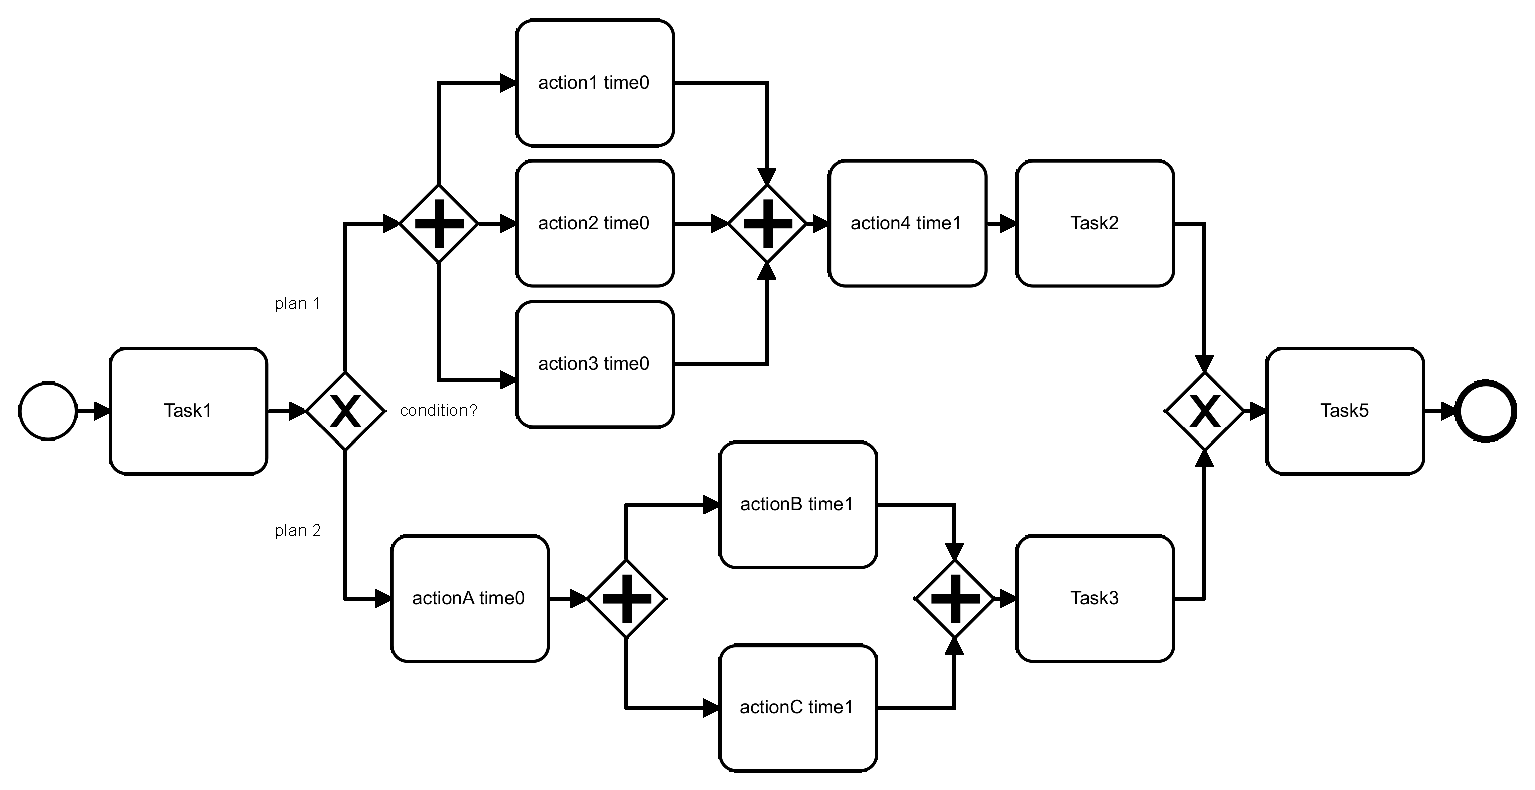
\includegraphics[width=\linewidth]{examplep.eps}
    	\caption{The Business Process Diagram after launching BPMNPA.}
  	\end{subfigure}
	\caption{An example of the execution results.}
	\label{fig:coffee}
\end{figure}